\documentclass[a4paper,12pt]{article}
%\documentclass[a4paper,fontsize=13pt]{scrartcl}

\usepackage{tabularx}
\usepackage{amsmath}
\usepackage[utf8]{inputenc}
\usepackage{multicol}
\usepackage{amsmath, amssymb, amsthm}
\usepackage{graphicx}
\usepackage{enumitem}
\usepackage{array}
\usepackage[left=2cm, right=2cm, top=2cm, bottom=2cm]{geometry}
\usepackage{fancyhdr}
\usepackage{xfp}
\usepackage{pgf}
\usepackage{tikz}

\usepackage{graphicx}
\usepackage{fancyhdr}
\setlength{\headheight}{28pt} % genug Platz für das Logo
\pagestyle{fancy}
\fancyhf{} % alles leeren
\fancyhead[L]{\includegraphics[height=1.2cm]{logo.png}}
\fancyhead[C]{\small Klassenarbeit – Potenzfunktionen \ (Kl. G10B)}
\fancyhead[R]{\small Name:\ \rule{2.8cm}{0.4pt}}
\fancyfoot[C]{\thepage}

\fancyfoot[C]{Seite \thepage \enspace\textbullet\enspace J.\,Mycan \textcopyright~2025 *Klassenarbeit 45 min.*}

\renewcommand{\footrulewidth}{0.4pt}




%\pagestyle{fancy}
%\lhead{Klassenarbeit 45min.}
%\chead{Heinrich-von-Kleist-Schule}
%\rhead{Mathematik - G8A}
%\lfoot{}
%\cfoot{Seite \thepage}
%\rfoot{}

\newcommand{\punkteA}{6}
\newcommand{\punkteB}{6}
\newcommand{\punkteC}{6}
\newcommand{\punkteD}{18}
\newcommand{\punkteE}{6}
%\newcommand{\punkteF}{12}

\newcommand{\maxSumme}{42}
\newcommand{\noteEinsMin}{\fpeval{round(\maxSumme * 0.95,0)}}
\newcommand{\noteZweiMin}{\fpeval{round(\maxSumme * 0.80,0)}}
\newcommand{\noteDreiMin}{\fpeval{round(\maxSumme * 0.60,0)}}
\newcommand{\noteVierMin}{\fpeval{round(\maxSumme * 0.45,0)}}
\newcommand{\noteFunfMin}{\fpeval{round(\maxSumme * 0.20,0)}}
\newcommand{\noteSechsMin}{0}

\newcommand{\summe}{%
	\pgfmathparse{\punkteA + \punkteB + \punkteC + \punkteD + \punkteE}%
	\pgfmathprintnumber{\pgfmathresult}}

\begin{document}
	
%	\begin{center}
%		\textbf{Klassenarbeit - Lineare Funktionen und LGS}
%	\end{center}
	
%	\textbf{Vor- und Nachname:} \underline{\hspace{10cm}}\\[0.1cm]
Die Lösungen sowie Lösungswege sollen klar strukturiert und gut nachvollziehbar sein. Zeige alle Zwischenschritte und markiere das Endergebnis deutlich. Vereinfache Ergebnisse soweit möglich. \\
	
	% -------------------------------------------------
	% Aufgabe 1
	% -------------------------------------------------
\textbf{Aufgabe 1 (6 Punkte)}\\
Bestimme zu den folgenden Angaben jeweils die Funktionsgleichung einer
quadratischen Funktion in \emph{Scheitelpunktform}.

\begin{enumerate}
	\item[a)] Gegeben ist der Scheitelpunkt der Normalparabel \(S(-2\mid 3)\). 
	Stelle die Funktionsgleichung dieser Parabel in Scheitelpunktform auf.
	
	\item[b)] Gegeben ist die quadratische Funktion 
	\[
	f(x) = -1{,}5x^{2} - 12x + 18.
	\]
	Bringe \(f(x)\) in die Scheitelpunktform.
	
	\item[c)] Eine quadratische Funktion \(g\) besitzt die Nullstellen 
	\(x_1 = -1\) und \(x_2 = 5\) und hat den Streckfaktor \(a = 2\).\\
	Bestimme eine Funktionsgleichung von \(g\) in Scheitelpunktform.
\end{enumerate}

\textbf{Lösung zu Aufgabe 1}\\[0.5em]
\begin{enumerate}
	\item[a)] \textbf{Gegeben:} Scheitelpunkt der Normalparabel \(S(-2\mid 3)\).
	
	\textit{Schritt 1: Allgemeine Scheitelpunktform notieren.}\\
	Eine quadratische Funktion in Scheitelpunktform hat allgemein die Form
	\[
	f(x) = a\,(x - x_S)^2 + y_S,
	\]
	wobei \(S(x_S\mid y_S)\) der Scheitelpunkt ist und \(a\) der Streckfaktor.\\[0.3em]
	Bei einer \emph{Normalparabel} gilt \(a = 1\).
	
	\textit{Schritt 2: Scheitelpunkt einsetzen.}\\
	Der Scheitel liegt bei \(S(-2\mid 3)\), also \(x_S = -2\) und \(y_S = 3\).
	Damit:
	\[
	f(x) = 1\cdot (x - (-2))^2 + 3.
	\]
	
	\textit{Schritt 3: Vorzeichen vereinfachen.}\\
	\[
	f(x) = (x + 2)^2 + 3.
	\]
	
	\textbf{Ergebnis:}
	\[
	\boxed{f(x) = (x + 2)^2 + 3}
	\]
	
	%%%%%%%%%%%%%%%%%%%%%%%%%%%%%%%%%%%%%%%%%%%%%%%%%%%%%%%
	
	\item[b)] Gegeben ist
	\[
	f(x) = -1{,}5x^{2} - 12x + 18.
	\]
	Gesucht ist die Scheitelpunktform.
	
	\textit{Schritt 1: Dezimalzahl in Bruch umschreiben.}\\
	\(-1{,}5 = -\frac{3}{2}\), also
	\[
	f(x) = -\frac{3}{2}x^{2} - 12x + 18.
	\]
	
	\textit{Schritt 2: Faktor vor \(x^2\) ausklammern.}\\

	Damit:
	\[
	f(x) = -\frac{3}{2}\bigl(x^{2} + 8x\bigr) + 18.
	\]
	
	\textit{Schritt 3: Quadratische Ergänzung im Inneren.}\\
	Wir ergänzen das Quadrat für \(x^{2} + 8x\):

	Also:
	\[
	f(x) = -\frac{3}{2}\left[(x+4)^{2} - 16\right] + 18.
	\]
	
	\textit{Schritt 4: Ausmultiplizieren und zusammenfassen.}\\
	Zuerst den Faktor \(-\frac{3}{2}\) verteilen:
	\[
	f(x) = -\frac{3}{2}(x+4)^{2}
	+ \frac{3}{2}\cdot 16
	+ 18.
	\]
	
	also
	\[
	f(x) = -\frac{3}{2}(x+4)^{2} + 42.
	\]
	
	\textbf{Ergebnis (Scheitelpunktform):}
	\[
	\boxed{f(x) = -\frac{3}{2}(x+4)^{2} + 42}
	\]
	(oder mit Dezimalzahl: \(\boxed{f(x) = -1{,}5\,(x+4)^{2} + 42}\)).
	
	%%%%%%%%%%%%%%%%%%%%%%%%%%%%%%%%%%%%%%%%%%%%%%%%%%%%%%%
	
	\item[c)] Gegeben:
	\[
	x_1 = -1, \quad x_2 = 5, \quad a = 2.
	\]
	Gesucht: Scheitelpunktform von \(g\).
	
	\textit{Schritt 1: Produktform aus Nullstellen aufstellen.}\\
	Für eine quadratische Funktion mit Nullstellen \(x_1, x_2\) gilt
	\[
	g(x) = a(x - x_1)(x - x_2).
	\]
	Einsetzen von \(a=2\), \(x_1=-1\), \(x_2=5\):
	\[
	g(x) = 2\bigl(x - (-1)\bigr)\bigl(x - 5\bigr)
	= 2(x+1)(x-5).
	\]
	
	\textit{Schritt 2: Scheitelpunkt bestimmen.}\\
	Bei einer quadratischen Funktion mit zwei Nullstellen liegt der Scheitelpunkt
	genau in der Mitte zwischen \(x_1\) und \(x_2\) auf der x-Achse:
	\[
	x_S = \frac{x_1 + x_2}{2}
	= \frac{-1 + 5}{2}
	= \frac{4}{2}
	= 2.
	\]
	Um die y-Koordinate des Scheitelpunkts zu finden, setzen wir \(x_S = 2\) in \(g(x)\) ein:
	\[
	g(2) = 2(2+1)(2-5)
	= 2\cdot 3 \cdot (-3)
	= 2\cdot (-9)
	= -18.
	\]
	Also liegt der Scheitelpunkt bei
	\[
	S(2\mid -18).
	\]
	
	\textit{Schritt 3: Scheitelpunktform aufstellen.}\\
	Allgemein:
	\[
	g(x) = a(x - x_S)^2 + y_S.
	\]
	Einsetzen von \(a = 2\), \(x_S = 2\), \(y_S = -18\):
	\[
	g(x) = 2(x - 2)^{2} - 18.
	\]
	
	\textbf{Ergebnis:}
	\[
	\boxed{g(x) = 2(x - 2)^{2} - 18}
	\]
	
\end{enumerate}


	% -------------------------------------------------
	% Aufgabe 2
	% -------------------------------------------------
	\textbf{Aufgabe 2 (Punkte)}\\
Ein Landwirt will an einer geraden Mauer einen rechteckigen Hühnerhof mit
Maschendraht abgrenzen. Die Mauer bildet dabei \emph{eine} Seite des
Rechtecks, für die keine Einzäunung benötigt wird. Es stehen insgesamt
\(20\,\text{m}\) Maschendraht zur Verfügung.

\medskip
Wie groß müssen die Seitenlängen des Rechtecks gewählt werden, damit die
Hühner möglichst viel Platz haben? Begründe dein Ergebnis.

\begin{center}
	\begin{minipage}[t]{0.45\textwidth}
		\centering
		% ggf. kleine Skizze des Rechtecks an der Mauer
		\includegraphics[width=\textwidth]{hof.png}
	\end{minipage}
\end{center}

\textbf{Lösung zu Aufgabe 2}\\[0.5em]

\textit{Ziel:} Die Seitenlängen des Rechtecks so wählen, dass die \emph{Fläche maximal} wird.


\textbf{Zaunlänge:} Es müssen nur drei Seiten eingezäunt werden:
\[
2x + y = 20.
\]

\bigskip
In Abhängigkeit von \(x\) ausdrücken.
\[
y = 20 - 2x.
\]

\bigskip
\textit{Schritt 3: Flächenfunktion \(A(x)\) aufstellen.}\\
Die Fläche des Rechtecks ist
\[
A = \text{Länge} \cdot \text{Breite} = x \cdot y.
\]
Wir setzen nun \(y = 20 - 2x\) ein:
\[
A(x) = x \cdot (20 - 2x).
\]
Jetzt ausmultiplizieren:
\[
A(x) = 20x - 2x^{2}.
\]

\medskip
Damit haben wir eine quadratische Funktion
\[
A(x) = -2x^{2} + 20x,
\]
die die Fläche in Abhängigkeit von \(x\) beschreibt.

\bigskip
\textit{Schritt 5: Maximum der Flächenfunktion bestimmen (Scheitelpunkt).}\\
Die Funktion
\[
A(x) = -2x^{2} + 20x
\]
ist eine nach unten geöffnete Parabel (\(a = -2 < 0\)), ihr Maximum liegt im Scheitelpunkt.

Für eine quadratische Funktion \(A(x) = ax^{2} + bx + c\) liegt der Scheitel bei
\[
x_S = -\frac{b}{2a}.
\]

Hier ist
\[
a = -2,\quad b = 20.
\]
Wir berechnen:
\[
x_S = -\frac{20}{2\cdot(-2)} = -\frac{20}{-4} = 5.
\]

\medskip
Also ist die optimale Tiefe des Hofes
\[
x = 5\,\text{m}.
\]

\bigskip
\textit{Schritt 6: Passende Länge \(y\) der Seite parallel zur Mauer bestimmen.}\\
Wir setzen \(x = 5\) in
\[
y = 20 - 2x
\]
ein:
\[
y = 20 - 2\cdot 5 = 20 - 10 = 10.
\]

\bigskip
\textit{Schritt 7: Maximale Fläche berechnen (optional zur Kontrolle).}\\
\[
A_{\max} = A(5) = 5\cdot 10 = 50\,\text{m}^2.
\]

\bigskip
\textbf{Antwortsatz:}\\
Die Hühner haben bei gegebenen \(20\,\text{m}\) Maschendraht am meisten Platz,
wenn die beiden Seiten senkrecht zur Mauer jeweils
\[
\boxed{5\,\text{m}}
\]
und die eingezäunte Seite parallel zur Mauer
\[
\boxed{10\,\text{m}}
\]
lang sind. Dann beträgt die maximale Fläche
\[
\boxed{50\,\text{m}^2}.
\]

	% -------------------------------------------------
	% Aufgabe 3
	% -------------------------------------------------
\textbf{Aufgabe 3 (6 Punkte)}\\
Begründe zunächst welche Art der Symmetrie liegt jeweils vor. Untersuche rechnerisch die folgenden Funktionen auf Symmetrie.  

\begin{enumerate}
		
	\item[a)] \(g(x) = \dfrac{1}{3}x^{5} - 2x^{3} + x\)
	
	\item[b)] \(f(x) = -\dfrac{1}{2}x^{-4} + 3x^{-2} + 1\)
	
	\item[c)] \(h(x) = \dfrac{1}{4}x^6 - \dfrac{1}{5}x^4 + \dfrac{1}{6}x^2 - 3x + 1\)
\end{enumerate}

\textbf{Lösung zu Aufgabe 3}\\[0.5em]
Gegeben sind die drei Funktionen. Wir prüfen jeweils die Symmetrie durch Einsetzen von \(-x\).

\medskip
\textit{Erinnerung:}
\begin{itemize}
	\item Achsensymmetrie zur \(y\)-Achse: \quad \(f(-x) = f(x)\) \quad (Funktion ist \emph{gerade}).
	\item Punktsymmetrie zum Ursprung: \quad \(f(-x) = -f(x)\) \quad (Funktion ist \emph{ungerade}).
\end{itemize}

\begin{enumerate}
	%%%%%%%%%%%%%%%%%%%%%%%%%%%%%%%%%%%%%%%%%%%%%%%%%%%%%%
	\item[a)] \(g(x) = \dfrac{1}{3}x^{5} - 2x^{3} + x\)
	
	\textit{Beobachtung:}  
	Alle Terme enthalten nur ungerade Potenzen von \(x\) (5, 3, 1) und keinen konstanten Term.  
	Das lässt eine Punktsymmetrie zum Ursprung vermuten.
	
	\medskip
	\textit{Rechnerischer Nachweis: \(g(-x)\) berechnen.}
	\[
	g(-x) = \frac{1}{3}(-x)^{5} - 2(-x)^{3} + (-x)
	\]

	somit:
	\[
	g(-x) = \frac{1}{3}\cdot(-x^{5}) - 2\cdot(-x^{3}) - x
	= -\frac{1}{3}x^{5} + 2x^{3} - x.
	\]
	
	Jetzt vergleichen wir mit \(-g(x)\):
	\[
	g(x) = \frac{1}{3}x^{5} - 2x^{3} + x
	\quad\Rightarrow\quad
	-g(x) = -\frac{1}{3}x^{5} + 2x^{3} - x.
	\]
	
	Man sieht:
	\[
	g(-x) = -g(x).
	\]
	
	\textbf{Ergebnis:}  
	\(\boxed{g(-x) = -g(x) \;\Rightarrow\; g \text{ ist ungerade und punktsymmetrisch zum Ursprung.}}\)
	
	%%%%%%%%%%%%%%%%%%%%%%%%%%%%%%%%%%%%%%%%%%%%%%%%%%%%%%
	\item[b)] \(f(x) = -\dfrac{1}{2}x^{-4} + 3x^{-2} + 1\)
		
	\medskip
	\textit{Rechnerischer Nachweis: \(f(-x)\) berechnen.}
	\[
	f(-x) = -\frac{1}{2}(-x)^{-4} + 3(-x)^{-2} + 1.
	\]
	
	Wir nutzen:
	\[
	(-x)^{-4} = \frac{1}{(-x)^{4}} = \frac{1}{x^{4}} = x^{-4},
	\qquad
	(-x)^{-2} = \frac{1}{(-x)^{2}} = \frac{1}{x^{2}} = x^{-2}.
	\]
	
	Damit:
	\[
	f(-x) = -\frac{1}{2}x^{-4} + 3x^{-2} + 1.
	\]
	
	Das ist genau der ursprüngliche Funktionsterm:
	\[
	f(-x) = f(x).
	\]
	
	\textbf{Ergebnis:}  
	\(\boxed{f(-x) = f(x) \;\Rightarrow\; f \text{ ist gerade und achsensymmetrisch zur } y\text{-Achse.}}\)
	
	%%%%%%%%%%%%%%%%%%%%%%%%%%%%%%%%%%%%%%%%%%%%%%%%%%%%%%
	\item[c)] \(h(x) = \dfrac{1}{4}x^6 - \dfrac{1}{5}x^4 + \dfrac{1}{6}x^2 - 3x + 1\)
	
	\textit{Beobachtung:}  
	\begin{itemize}
		\item Die Terme \(\frac{1}{4}x^6\), \(-\frac{1}{5}x^4\), \(\frac{1}{6}x^2\) und \(+1\) enthalten nur gerade Potenzen bzw. eine Konstante.
		\item Der Term \(-3x\) hat eine ungerade Potenz.
	\end{itemize}
	Es ist also eine Mischung aus geraden und ungeraden Anteilen → Verdacht: \emph{keine} Symmetrie.

	
\end{enumerate}

	% -------------------------------------------------
	% Aufgabe 4
	% -------------------------------------------------
\textbf{Aufgabe 4 (18 Punkte)}\\
Löse die folgenden Potenzgleichungen. Vereinfache jeweils sinnvoll und gib alle Lösungen an.

\[
\begin{aligned}
	\text{a)}\quad & 2^{x+2} - 8 \;=\; 3\cdot 2^{x-1} \\[4pt]
	\text{b)}\quad & 3^{x+1} + 3^{x} \;=\; 36 \\[4pt]
	\text{c)}\quad & 5^{2x-1} \;=\; 125\cdot 5^{x-3} \\[4pt]
	\text{d)}\quad & \left(\frac{1}{2}\right)^{x-2} + \left(\frac{1}{2}\right)^{x}
	\;=\; 5\cdot \left(\frac{1}{2}\right)^{x+1}
\end{aligned}
\]

\textbf{Lösung zu Aufgabe 4}\\[0.5em]
Gegeben sind die Potenzgleichungen. Gesucht sind alle reellen Lösungen.

\[
\begin{aligned}
	\text{a)}\quad & 5^{x+1} + 25 \;=\; 6\cdot 5^{x} \\[2pt]
	\text{b)}\quad & 3^{x+1} + 3^{x} = 36 \\[2pt]
	\text{c)}\quad & 5^{2x-1} = 125\cdot 5^{x-3} \\[2pt]
	\text{d)}\quad & \left(\frac{1}{2}\right)^{x-2} + \left(\frac{1}{2}\right)^{x}
	= 5\cdot \left(\frac{1}{2}\right)^{x+1}
\end{aligned}
\]
	% -------------------------------------------------
	% Aufgabe 5
	% -------------------------------------------------
\textbf{Aufgabe 5 ( Punkte)}\\
Welche der angegebenen Funktionsgleichungen passt jeweils zum dargestellten Graphen?
Begründe deine Wahl.

\begin{center}
	\begin{tabular}{cc}
		
		% =========================================
		% BLOCK 1 (oben links): Kubische Funktion
		% =========================================
		\begin{minipage}[t]{0.45\textwidth}
			% linke Minipage: Graph
			\begin{minipage}[t]{0.58\textwidth}
				\begin{tikzpicture}[scale=0.8]
					% Koordinatensystem: x von -1 bis 4, y von -2 bis 4
					\draw[step=0.5,very thick,gray!60] (-1,-2) grid (4,4);
					\draw[->] (-1,0) -- (4.2,0) node[right] {$x$};
					\draw[->] (0,-2) -- (0,4.2) node[above] {$y$};
					% Ticks
					\foreach \x in {-1,0,1,2,3,4}
					\draw (\x,0.1) -- (\x,-0.1);
					\foreach \y in {-2,-1,1,2,3,4}
					\draw (0.1,\y) -- (-0.1,\y);
					% Graph: f(x) = 1.5 (x-1)^3 + 1
					% Domain so gewählt, dass y zwischen etwa -2 und 4 bleibt
					\draw[domain=-0.25:2.25,smooth,thick,variable=\x]
					plot ({\x},{-1.5*(\x-1)*(\x-1)*(\x-1) + 1});
				\end{tikzpicture}
			\end{minipage}%
			\hfill
			% rechte Minipage: Funktionsauswahl
			\begin{minipage}[t]{0.42\textwidth}
				\scriptsize
				\begin{tabular}{@{}l@{}}
					a) $f(x) = -1{,}5(x-1)^{3} + 1$\\[2pt]
					b) $f(x) = -1{,}5(x+1)^{3} + 1$\\[2pt]
					c) $f(x) = -1{,}5(x-1)^{3} - 1$\\[2pt]
					d) $f(x) = 0{,}5(x-1)^{3} + 1$
				\end{tabular}
			\end{minipage}
		\end{minipage}
		&
		% =========================================
		% BLOCK 2 (oben rechts): Potenzfunktion 1/x^4
		% =========================================
		\begin{minipage}[t]{0.45\textwidth}
			% linke Minipage: Graph
			\begin{minipage}[t]{0.58\textwidth}
				\begin{tikzpicture}[scale=0.8]
					\draw[step=0.5,thick,gray!60] (-4,-2) grid (4,4);
					\draw[->] (-4,0) -- (4.2,0) node[right] {$x$};
					\draw[->] (0,-2) -- (0,2.2) node[above] {$y$};
					\foreach \x in {-4,-3,-2,-1,1,2,3,4}
					\draw (\x,0.1) -- (\x,-0.1);
					\foreach \y in {-2,-1,1,2}
					\draw (0.1,\y) -- (-0.1,\y);
					% Graph: f(x) = 2/x^4 - 1, |x| >= 0.8 (damit alles im Bild bleibt)
					\draw[domain=-4:-0.8,smooth,thick,variable=\x]
					plot ({\x},{2/(\x*\x*\x*\x) - 1});
					\draw[domain=0.8:4,smooth,thick,variable=\x]
					plot ({\x},{2/(\x*\x*\x*\x) - 1});
				\end{tikzpicture}
			\end{minipage}%
			\hfill
			% rechte Minipage: Funktionsauswahl
			\begin{minipage}[t]{0.20\textwidth}
				\scriptsize
				\begin{tabular}{@{}l@{}}
					a) $f(x) = 2\dfrac{1}{x^{4}} - 1$\\[2pt]
					b) $f(x) = -2\dfrac{1}{x^{4}} - 1$\\[2pt]
					c) $f(x) = \dfrac{2}{x^{2}} - 1$\\[2pt]
					d) $f(x) = \dfrac{2}{x^{4}} + 1$
				\end{tabular}
			\end{minipage}
		\end{minipage}
		\\[1.4cm]
		
		% =========================================
		% BLOCK 3 (unten links): Wurzelfunktion
		% =========================================
		\begin{minipage}[t]{0.45\textwidth}
			\begin{minipage}[t]{0.58\textwidth}
				\begin{tikzpicture}[scale=0.8]
					\draw[step=0.5,very thick,gray!60] (0,-1) grid (5,4);
					\draw[->] (0,-1) -- (5.2,-1) node[right] {$x$};
					\draw[->] (0,-1) -- (0,4.2) node[above] {$y$};
					\foreach \x in {0,1,2,3,4,5}
					\draw (\x,-0.9) -- (\x,-1.1);
					\foreach \y in {-1,0,1,2,3,4}
					\draw (0.1,\y) -- (-0.1,\y);
					% Graph: f(x) = sqrt(x) + 1
					\draw[domain=0:5,smooth,thick,variable=\x]
					plot ({\x},{sqrt(\x)+1});
				\end{tikzpicture}
			\end{minipage}%
			\hfill
			\begin{minipage}[t]{0.38\textwidth}
				\scriptsize
				\begin{tabular}{@{}l@{}}
					a) $f(x) = \sqrt{x} + 1$\\[2pt]
					b) $f(x) = \sqrt{x-1} + 1$\\[2pt]
					c) $f(x) = \sqrt{x} - 1$\\[2pt]
					d) $f(x) = 2\sqrt{x} + 1$
				\end{tabular}
			\end{minipage}
		\end{minipage}
		&
		% =========================================
		% BLOCK 4 (unten rechts): Kubikwurzel-Funktion
		% =========================================
		\begin{minipage}[t]{0.45\textwidth}
			\begin{minipage}[t]{0.58\textwidth}
				\begin{tikzpicture}[scale=0.8]
					\draw[step=0.5,thick,gray!60] (-4,-3) grid (4,2);
					\draw[->] (-4,0) -- (4.2,0) node[right] {$x$};
					\draw[->] (0,-2) -- (0,2.2) node[above] {$y$};
					\foreach \x in {-4,-3,-2,-1,1,2,3,4}
					\draw (\x,0.1) -- (\x,-0.1);
					\foreach \y in {-2,-1,1,2}
					\draw (0.1,\y) -- (-0.1,\y);
					% Graph: f(x) = x^(1/3) - 1
					\draw[domain=-4:4,smooth,thick,variable=\x]
					plot ({\x},{sign(\x)*abs(\x)^(1/3) - 1});
				\end{tikzpicture}
			\end{minipage}%
			\hfill
			\begin{minipage}[t]{0.20\textwidth}
				\scriptsize
				\begin{tabular}{@{}l@{}}
					a) $f(x) = \dfrac{x}{x^{3}} - 1$\\[2pt]
					b) $f(x) = -x^{\dfrac{1}{3}} - 1$\\[2pt]
					c) $f(x) = x^{\dfrac{1}{3}} - 1$\\[2pt]
					d) $f(x) = \dfrac{1}{|x^{2}|} + 1$
				\end{tabular}
			\end{minipage}
		\end{minipage}
		
	\end{tabular}
\end{center}

	
	\textbf{Notenschlüssel:}
	\begin{center}
		\begin{tabular}{|c|c|c|c|c|c|c|}
			\hline
			Note & 1 & 2 & 3 & 4 & 5 & 6 \\
			\hline
			Prozent \% & 100--95 & 94--80 & 79--60 & 59--45 & 44--16 & 15--0 \\
			\hline
			Punkte & \maxSumme{}--\noteEinsMin{} & \fpeval{\noteEinsMin-1}--\noteZweiMin{} & \fpeval{\noteZweiMin-1}--\noteDreiMin{} & \fpeval{\noteDreiMin-1}--\noteVierMin{} & \fpeval{\noteVierMin-1}--\noteFunfMin{} & \fpeval{\noteFunfMin-1}--\noteSechsMin{} \\
			\hline
		\end{tabular}
	\end{center}
	
	\vspace{2cm}
	\textbf{Kenntnisnahme eines Elternteils:} \hrulefill \hfill \textbf{Note:} \hrulefill
	
\end{document}
